\documentclass[tikz, border = 10pt]{standalone}

\usepackage{newpxtext,newpxmath}   % /upbeta
%\usepackage{fouriernc}            % /otherbeta
\usepackage{amsmath}
\renewcommand{\familydefault}{\sfdefault}
\usepackage{mathastext}

\usetikzlibrary{positioning, quotes, calc, math, arrows.meta, bending, shapes, backgrounds}

\tikzset{
every edge quotes/.style = {fill = white},
every node/.style = {scale = 1.1},
manifest/.style = {rectangle, draw, thin, inner sep = 3pt, minimum width = 1cm,
   minimum height = .85cm, align = center},
latent/.style = {ellipse, draw, thin, inner sep = 3pt, minimum width = 1cm,
   minimum height = .85cm},
residual1/.style = {circle, draw, thin, minimum size = 5mm, inner sep = 1pt},
residual2/.style = {rectangle, minimum width = 0.5pt, minimum height = 1.5mm,
   inner sep = 0pt, outer sep = 0mm},
regression/.style = {-{Stealth[length = 1.5mm]}, thin, shorten > = 1pt, 
   inner sep = 1.5pt, outer sep = 0mm},
covariance/.style={{Stealth[length = 1.5mm]}-{Stealth[length = 1.5mm]}, thin,
   shorten > = 1pt, shorten < = 1pt, inner sep = 1.5pt},
variance/.style={{Stealth[length = 1mm]}-{Stealth[length = 1mm]}, thin,
   shorten > = 1pt, shorten < = 1pt, inner sep = 1pt},
interaction/.style = {-{Stealth[sep = 1pt, length = 1.5mm] . Circle[length = 4pt]},
   thin, shorten > = -2pt},
constant/.style = {draw, thin, inner sep = 1pt, regular polygon,
   regular polygon sides = 3, minimum size = 5mm},
group/.style = {rectangle, inner sep = 2pt, minimum width = 15mm, minimum height = 5mm, 
   align = center}
}

\begin{document}
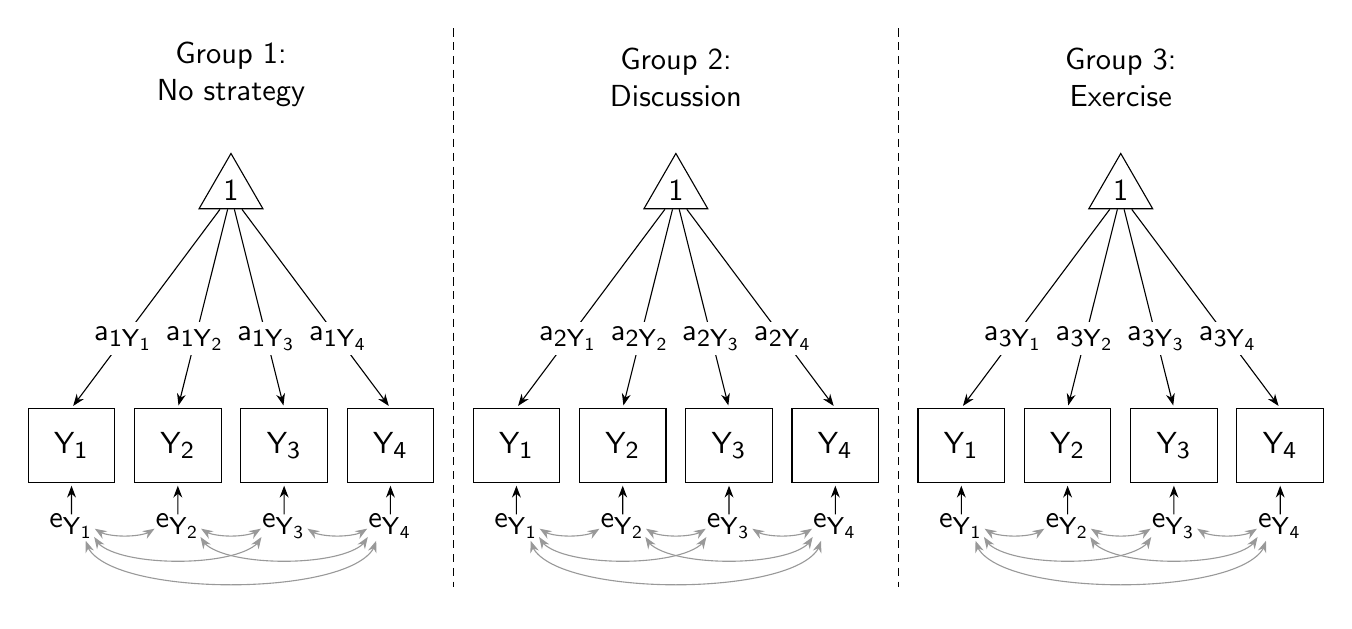
\begin{tikzpicture}

%% Dependents and their residuals
\foreach \i [remember = \x as \lastx (initially 0)] in {1,...,12}{
   \tikzmath{\labnum = int(mod(\i - 1, 4) + 1);} 
   \node [manifest] (y\i) at (\lastx, 0) {Y$_{\labnum}$};
   \node [residual2] (e\i) [below = 4mm of y\i] {e$_{Y_\labnum}$};
   \path [regression] (e\i) edge (y\i);  
   \ifnum \labnum = 4  \def\d{0.5} \else \def\d{0.25} \fi   
   \tikzmath{\x = \lastx + \d + 1.1;} 
}

\foreach \i/\j in {1/No strategy, 2/Discussion, 3/Exercise} {
   %% Means
   \tikzmath{\ya = int((\i - 1)*4 + 2);} 
   \tikzmath{\yb = int(\ya + 1);} 
   \node [constant] (const\i) [above = 3cm of $(y\ya)!0.5!(y\yb)$] {1};
   \foreach \b/\c in {1/240, 2/260, 3/280, 4/300} {
      \tikzmath{\d = int((\i - 1)*4 + \b);} 
      \path [regression] (const\i.\c) edge ["a$_{\i{Y_\b}}$", pos = 0.65] (y\d.90);
   }

   %% Groups
   \node [group] (gp\i) [above = 0.5cm of const\i] {Group \i:\\\j};
}

%% Covariances
\newcommand{\eout}{{0, 340, 320}}     % out angle
\newcommand{\ein}{{180, 200, 220}}    % in angle
\newcommand{\bend}{{80, 85, 90}}      % bend

\foreach \g in {1,5,9}                % three groups of four variables - label for first in each group
   \foreach \i in {1,2,3}                             
      \foreach \j [parse = true] in {\i+1,...,4}{     
        \tikzmath{\idash = int(\g + \i - 1);  \jdash = int(\g + \j - 1);}    % out and in labels for e
        \tikzmath{\index = \j - \i - 1;}                                     % array element
        \tikzmath{\first = \eout[\index]; \second = \ein[\index]; \third = \bend[\index];}
        \path [covariance, black!40] (e\idash.\first) edge [bend right = \third, looseness = 0.55,] (e\jdash.\second); 
}

%% Separators
\foreach \i in {4,8} {
   \tikzmath{\j = int(\i + 1);}
   \coordinate (M) at ($(y\i)!0.5!(y\j)$);
   \draw [style = densely dashed, thin] ($(M)!5.3cm!270:(y\i)$) -- ($(M)!1.8cm!90:(y\i)$);
}

\end{tikzpicture}
\end{document}